\clearpage
\onecolumn
\section{All Authored Models: Scored Case Studies}
These are constructed positive and negative evaluator controls, not model predictions.
The 18 source models remain 18 sources; their 36 demonstration cases are not independent samples.
All 5,120 frozen procedural sources are shown separately in the 80-page offline gallery.
\subsection{Garden Bench}
\noindent Source: \texttt{easy-garden-bench}.
Two cases share this source. Read numeric/graph answer fields alongside context-only images.
\paragraph{plan.} Case \texttt{152306ac476e4708d75f7668}.\par
Given the full target, return all IDs in an executable vertical insertion order. The negative reverses the order.\par
\noindent\begin{tabular}{@{}ccc@{}}
Input / context & Positive reference & Constructed negative\\

\includegraphics[width=.31\textwidth]{figures/review-cases/case-01-input.jpg} & 
\includegraphics[width=.31\textwidth]{figures/review-cases/case-01-good.jpg} & 
\includegraphics[width=.31\textwidth]{figures/review-cases/case-01-bad.jpg}\\
\end{tabular}\par
\noindent Strict success: positive $1$, negative $0$. Rejection: \texttt{unsupported, incomplete}.
Machine-readable inputs, both answers and all metrics are in \texttt{review-gallery/case-01.json}.
Field-answer cases use scene images for context only; a matching scene is not a correct field answer.
\paragraph{repair.} Case \texttt{3a48a42a7c4f4265c5bc9d3a}.\par
Given current and full symbolic reference, restore a wrong color and report its current ID. The negative copies current.\par
\noindent\begin{tabular}{@{}ccc@{}}
Input / context & Positive reference & Constructed negative\\

\includegraphics[width=.31\textwidth]{figures/review-cases/case-02-input.jpg} & 
\includegraphics[width=.31\textwidth]{figures/review-cases/case-02-good.jpg} & 
\includegraphics[width=.31\textwidth]{figures/review-cases/case-02-bad.jpg}\\
\end{tabular}\par
\noindent Strict success: positive $1$, negative $0$. Rejection: \texttt{target\_mismatch}.
Machine-readable inputs, both answers and all metrics are in \texttt{review-gallery/case-02.json}.
Field-answer cases use scene images for context only; a matching scene is not a correct field answer.
\clearpage
\subsection{Four-Step Staircase}
\noindent Source: \texttt{easy-staircase}.
Two cases share this source. Read numeric/graph answer fields alongside context-only images.
\paragraph{plan.} Case \texttt{f6d7ad54390ef8403fa59152}.\par
Given the full target, return all IDs in an executable vertical insertion order. The negative reverses the order.\par
\noindent\begin{tabular}{@{}ccc@{}}
Input / context & Positive reference & Constructed negative\\

\includegraphics[width=.31\textwidth]{figures/review-cases/case-03-input.jpg} & 
\includegraphics[width=.31\textwidth]{figures/review-cases/case-03-good.jpg} & 
\includegraphics[width=.31\textwidth]{figures/review-cases/case-03-bad.jpg}\\
\end{tabular}\par
\noindent Strict success: positive $1$, negative $0$. Rejection: \texttt{unsupported, incomplete}.
Machine-readable inputs, both answers and all metrics are in \texttt{review-gallery/case-03.json}.
Field-answer cases use scene images for context only; a matching scene is not a correct field answer.
\paragraph{repair.} Case \texttt{cf27b03347e69a62e88adb00}.\par
Given current and full symbolic reference, restore a wrong color and report its current ID. The negative copies current.\par
\noindent\begin{tabular}{@{}ccc@{}}
Input / context & Positive reference & Constructed negative\\

\includegraphics[width=.31\textwidth]{figures/review-cases/case-04-input.jpg} & 
\includegraphics[width=.31\textwidth]{figures/review-cases/case-04-good.jpg} & 
\includegraphics[width=.31\textwidth]{figures/review-cases/case-04-bad.jpg}\\
\end{tabular}\par
\noindent Strict success: positive $1$, negative $0$. Rejection: \texttt{target\_mismatch}.
Machine-readable inputs, both answers and all metrics are in \texttt{review-gallery/case-04.json}.
Field-answer cases use scene images for context only; a matching scene is not a correct field answer.
\clearpage
\subsection{Garden Gate}
\noindent Source: \texttt{easy-garden-gate}.
Two cases share this source. Read numeric/graph answer fields alongside context-only images.
\paragraph{plan.} Case \texttt{3ba7340d88ba53b511995760}.\par
Given the full target, return all IDs in an executable vertical insertion order. The negative reverses the order.\par
\noindent\begin{tabular}{@{}ccc@{}}
Input / context & Positive reference & Constructed negative\\

\includegraphics[width=.31\textwidth]{figures/review-cases/case-05-input.jpg} & 
\includegraphics[width=.31\textwidth]{figures/review-cases/case-05-good.jpg} & 
\includegraphics[width=.31\textwidth]{figures/review-cases/case-05-bad.jpg}\\
\end{tabular}\par
\noindent Strict success: positive $1$, negative $0$. Rejection: \texttt{unsupported, incomplete}.
Machine-readable inputs, both answers and all metrics are in \texttt{review-gallery/case-05.json}.
Field-answer cases use scene images for context only; a matching scene is not a correct field answer.
\paragraph{repair.} Case \texttt{f1e7a66185b2390ffaec600f}.\par
Given current and full symbolic reference, restore a wrong color and report its current ID. The negative copies current.\par
\noindent\begin{tabular}{@{}ccc@{}}
Input / context & Positive reference & Constructed negative\\

\includegraphics[width=.31\textwidth]{figures/review-cases/case-06-input.jpg} & 
\includegraphics[width=.31\textwidth]{figures/review-cases/case-06-good.jpg} & 
\includegraphics[width=.31\textwidth]{figures/review-cases/case-06-bad.jpg}\\
\end{tabular}\par
\noindent Strict success: positive $1$, negative $0$. Rejection: \texttt{target\_mismatch}.
Machine-readable inputs, both answers and all metrics are in \texttt{review-gallery/case-06.json}.
Field-answer cases use scene images for context only; a matching scene is not a correct field answer.
\clearpage
\subsection{Picnic Table}
\noindent Source: \texttt{easy-picnic-table}.
Two cases share this source. Read numeric/graph answer fields alongside context-only images.
\paragraph{plan.} Case \texttt{c9ef6834c5de4d543be5b056}.\par
Given the full target, return all IDs in an executable vertical insertion order. The negative reverses the order.\par
\noindent\begin{tabular}{@{}ccc@{}}
Input / context & Positive reference & Constructed negative\\

\includegraphics[width=.31\textwidth]{figures/review-cases/case-07-input.jpg} & 
\includegraphics[width=.31\textwidth]{figures/review-cases/case-07-good.jpg} & 
\includegraphics[width=.31\textwidth]{figures/review-cases/case-07-bad.jpg}\\
\end{tabular}\par
\noindent Strict success: positive $1$, negative $0$. Rejection: \texttt{unsupported, incomplete}.
Machine-readable inputs, both answers and all metrics are in \texttt{review-gallery/case-07.json}.
Field-answer cases use scene images for context only; a matching scene is not a correct field answer.
\paragraph{repair.} Case \texttt{92deb3d852a09a10aac8b5c4}.\par
Given current and full symbolic reference, restore a wrong color and report its current ID. The negative copies current.\par
\noindent\begin{tabular}{@{}ccc@{}}
Input / context & Positive reference & Constructed negative\\

\includegraphics[width=.31\textwidth]{figures/review-cases/case-08-input.jpg} & 
\includegraphics[width=.31\textwidth]{figures/review-cases/case-08-good.jpg} & 
\includegraphics[width=.31\textwidth]{figures/review-cases/case-08-bad.jpg}\\
\end{tabular}\par
\noindent Strict success: positive $1$, negative $0$. Rejection: \texttt{target\_mismatch}.
Machine-readable inputs, both answers and all metrics are in \texttt{review-gallery/case-08.json}.
Field-answer cases use scene images for context only; a matching scene is not a correct field answer.
\clearpage
\subsection{Canal Bridge}
\noindent Source: \texttt{medium-canal-bridge}.
Two cases share this source. Read numeric/graph answer fields alongside context-only images.
\paragraph{plan.} Case \texttt{5c96ed823332734ad4af5053}.\par
Given the full target, return all IDs in an executable vertical insertion order. The negative reverses the order.\par
\noindent\begin{tabular}{@{}ccc@{}}
Input / context & Positive reference & Constructed negative\\

\includegraphics[width=.31\textwidth]{figures/review-cases/case-09-input.jpg} & 
\includegraphics[width=.31\textwidth]{figures/review-cases/case-09-good.jpg} & 
\includegraphics[width=.31\textwidth]{figures/review-cases/case-09-bad.jpg}\\
\end{tabular}\par
\noindent Strict success: positive $1$, negative $0$. Rejection: \texttt{unsupported, incomplete}.
Machine-readable inputs, both answers and all metrics are in \texttt{review-gallery/case-09.json}.
Field-answer cases use scene images for context only; a matching scene is not a correct field answer.
\paragraph{repair.} Case \texttt{62c0448ef5755ddb2d3e7ad4}.\par
Given current and full symbolic reference, restore a wrong color and report its current ID. The negative copies current.\par
\noindent\begin{tabular}{@{}ccc@{}}
Input / context & Positive reference & Constructed negative\\

\includegraphics[width=.31\textwidth]{figures/review-cases/case-10-input.jpg} & 
\includegraphics[width=.31\textwidth]{figures/review-cases/case-10-good.jpg} & 
\includegraphics[width=.31\textwidth]{figures/review-cases/case-10-bad.jpg}\\
\end{tabular}\par
\noindent Strict success: positive $1$, negative $0$. Rejection: \texttt{target\_mismatch}.
Machine-readable inputs, both answers and all metrics are in \texttt{review-gallery/case-10.json}.
Field-answer cases use scene images for context only; a matching scene is not a correct field answer.
\clearpage
\subsection{Park Pavilion}
\noindent Source: \texttt{medium-pavilion}.
Two cases share this source. Read numeric/graph answer fields alongside context-only images.
\paragraph{plan.} Case \texttt{025e602d17a4226de90cdd8e}.\par
Given the full target, return all IDs in an executable vertical insertion order. The negative reverses the order.\par
\noindent\begin{tabular}{@{}ccc@{}}
Input / context & Positive reference & Constructed negative\\

\includegraphics[width=.31\textwidth]{figures/review-cases/case-11-input.jpg} & 
\includegraphics[width=.31\textwidth]{figures/review-cases/case-11-good.jpg} & 
\includegraphics[width=.31\textwidth]{figures/review-cases/case-11-bad.jpg}\\
\end{tabular}\par
\noindent Strict success: positive $1$, negative $0$. Rejection: \texttt{unsupported, incomplete}.
Machine-readable inputs, both answers and all metrics are in \texttt{review-gallery/case-11.json}.
Field-answer cases use scene images for context only; a matching scene is not a correct field answer.
\paragraph{repair.} Case \texttt{ff174846fe2b77b68cafa0b1}.\par
Given current and full symbolic reference, restore a wrong color and report its current ID. The negative copies current.\par
\noindent\begin{tabular}{@{}ccc@{}}
Input / context & Positive reference & Constructed negative\\

\includegraphics[width=.31\textwidth]{figures/review-cases/case-12-input.jpg} & 
\includegraphics[width=.31\textwidth]{figures/review-cases/case-12-good.jpg} & 
\includegraphics[width=.31\textwidth]{figures/review-cases/case-12-bad.jpg}\\
\end{tabular}\par
\noindent Strict success: positive $1$, negative $0$. Rejection: \texttt{target\_mismatch}.
Machine-readable inputs, both answers and all metrics are in \texttt{review-gallery/case-12.json}.
Field-answer cases use scene images for context only; a matching scene is not a correct field answer.
\clearpage
\subsection{Townhouse}
\noindent Source: \texttt{medium-townhouse}.
Two cases share this source. Read numeric/graph answer fields alongside context-only images.
\paragraph{plan.} Case \texttt{39fc27ace5ece93b349ee3a8}.\par
Given the full target, return all IDs in an executable vertical insertion order. The negative reverses the order.\par
\noindent\begin{tabular}{@{}ccc@{}}
Input / context & Positive reference & Constructed negative\\

\includegraphics[width=.31\textwidth]{figures/review-cases/case-13-input.jpg} & 
\includegraphics[width=.31\textwidth]{figures/review-cases/case-13-good.jpg} & 
\includegraphics[width=.31\textwidth]{figures/review-cases/case-13-bad.jpg}\\
\end{tabular}\par
\noindent Strict success: positive $1$, negative $0$. Rejection: \texttt{unsupported, incomplete}.
Machine-readable inputs, both answers and all metrics are in \texttt{review-gallery/case-13.json}.
Field-answer cases use scene images for context only; a matching scene is not a correct field answer.
\paragraph{repair.} Case \texttt{04131146e62411747ad0ebc5}.\par
Given current and full symbolic reference, restore a wrong color and report its current ID. The negative copies current.\par
\noindent\begin{tabular}{@{}ccc@{}}
Input / context & Positive reference & Constructed negative\\

\includegraphics[width=.31\textwidth]{figures/review-cases/case-14-input.jpg} & 
\includegraphics[width=.31\textwidth]{figures/review-cases/case-14-good.jpg} & 
\includegraphics[width=.31\textwidth]{figures/review-cases/case-14-bad.jpg}\\
\end{tabular}\par
\noindent Strict success: positive $1$, negative $0$. Rejection: \texttt{target\_mismatch}.
Machine-readable inputs, both answers and all metrics are in \texttt{review-gallery/case-14.json}.
Field-answer cases use scene images for context only; a matching scene is not a correct field answer.
\clearpage
\subsection{Watchtower}
\noindent Source: \texttt{medium-watchtower}.
Two cases share this source. Read numeric/graph answer fields alongside context-only images.
\paragraph{plan.} Case \texttt{403b52f444583f361b1d37f3}.\par
Given the full target, return all IDs in an executable vertical insertion order. The negative reverses the order.\par
\noindent\begin{tabular}{@{}ccc@{}}
Input / context & Positive reference & Constructed negative\\

\includegraphics[width=.31\textwidth]{figures/review-cases/case-15-input.jpg} & 
\includegraphics[width=.31\textwidth]{figures/review-cases/case-15-good.jpg} & 
\includegraphics[width=.31\textwidth]{figures/review-cases/case-15-bad.jpg}\\
\end{tabular}\par
\noindent Strict success: positive $1$, negative $0$. Rejection: \texttt{unsupported, incomplete}.
Machine-readable inputs, both answers and all metrics are in \texttt{review-gallery/case-15.json}.
Field-answer cases use scene images for context only; a matching scene is not a correct field answer.
\paragraph{repair.} Case \texttt{6d49bea3c782adb17f8760c0}.\par
Given current and full symbolic reference, restore a wrong color and report its current ID. The negative copies current.\par
\noindent\begin{tabular}{@{}ccc@{}}
Input / context & Positive reference & Constructed negative\\

\includegraphics[width=.31\textwidth]{figures/review-cases/case-16-input.jpg} & 
\includegraphics[width=.31\textwidth]{figures/review-cases/case-16-good.jpg} & 
\includegraphics[width=.31\textwidth]{figures/review-cases/case-16-bad.jpg}\\
\end{tabular}\par
\noindent Strict success: positive $1$, negative $0$. Rejection: \texttt{target\_mismatch}.
Machine-readable inputs, both answers and all metrics are in \texttt{review-gallery/case-16.json}.
Field-answer cases use scene images for context only; a matching scene is not a correct field answer.
\clearpage
\subsection{Double-Span Bridge}
\noindent Source: \texttt{hard-double-span-bridge}.
Two cases share this source. Read numeric/graph answer fields alongside context-only images.
\paragraph{plan.} Case \texttt{dfacbf9787f98c34c8203850}.\par
Given the full target, return all IDs in an executable vertical insertion order. The negative reverses the order.\par
\noindent\begin{tabular}{@{}ccc@{}}
Input / context & Positive reference & Constructed negative\\
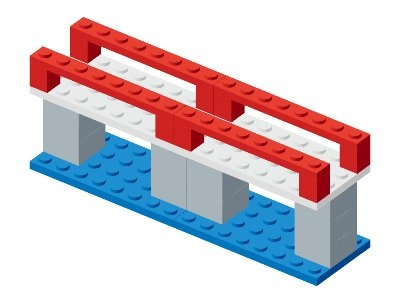
\includegraphics[width=.31\textwidth]{figures/review-cases/case-17-input.jpg} & 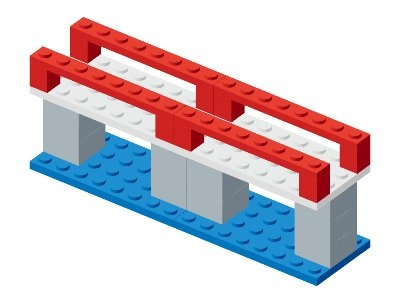
\includegraphics[width=.31\textwidth]{figures/review-cases/case-17-good.jpg} & 
\includegraphics[width=.31\textwidth]{figures/review-cases/case-17-bad.jpg}\\
\end{tabular}\par
\noindent Strict success: positive $1$, negative $0$. Rejection: \texttt{unsupported, incomplete}.
Machine-readable inputs, both answers and all metrics are in \texttt{review-gallery/case-17.json}.
Field-answer cases use scene images for context only; a matching scene is not a correct field answer.
\paragraph{repair.} Case \texttt{bb95cd1c7931fd1e15402b73}.\par
Given current and full symbolic reference, restore a wrong color and report its current ID. The negative copies current.\par
\noindent\begin{tabular}{@{}ccc@{}}
Input / context & Positive reference & Constructed negative\\
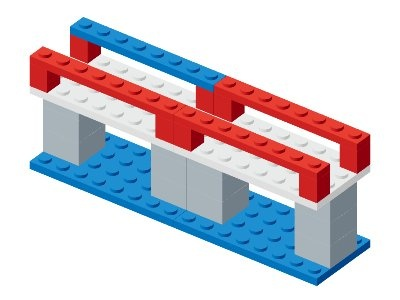
\includegraphics[width=.31\textwidth]{figures/review-cases/case-18-input.jpg} & 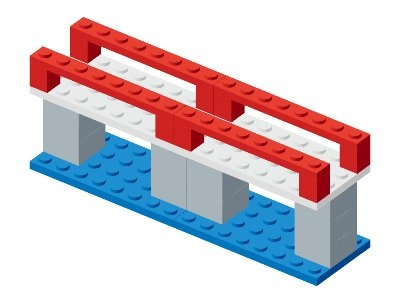
\includegraphics[width=.31\textwidth]{figures/review-cases/case-18-good.jpg} & 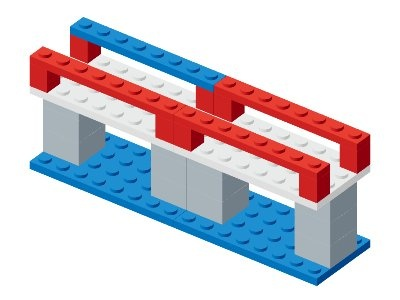
\includegraphics[width=.31\textwidth]{figures/review-cases/case-18-bad.jpg}\\
\end{tabular}\par
\noindent Strict success: positive $1$, negative $0$. Rejection: \texttt{target\_mismatch}.
Machine-readable inputs, both answers and all metrics are in \texttt{review-gallery/case-18.json}.
Field-answer cases use scene images for context only; a matching scene is not a correct field answer.
\clearpage
\subsection{Lighthouse}
\noindent Source: \texttt{hard-lighthouse}.
Two cases share this source. Read numeric/graph answer fields alongside context-only images.
\paragraph{plan.} Case \texttt{2ae74752a90a40fcc98cbb78}.\par
Given the full target, return all IDs in an executable vertical insertion order. The negative reverses the order.\par
\noindent\begin{tabular}{@{}ccc@{}}
Input / context & Positive reference & Constructed negative\\

\includegraphics[width=.31\textwidth]{figures/review-cases/case-19-input.jpg} & 
\includegraphics[width=.31\textwidth]{figures/review-cases/case-19-good.jpg} & 
\includegraphics[width=.31\textwidth]{figures/review-cases/case-19-bad.jpg}\\
\end{tabular}\par
\noindent Strict success: positive $1$, negative $0$. Rejection: \texttt{unsupported, incomplete}.
Machine-readable inputs, both answers and all metrics are in \texttt{review-gallery/case-19.json}.
Field-answer cases use scene images for context only; a matching scene is not a correct field answer.
\paragraph{repair.} Case \texttt{52cdc0d3b4abf89218b9254e}.\par
Given current and full symbolic reference, restore a wrong color and report its current ID. The negative copies current.\par
\noindent\begin{tabular}{@{}ccc@{}}
Input / context & Positive reference & Constructed negative\\

\includegraphics[width=.31\textwidth]{figures/review-cases/case-20-input.jpg} & 
\includegraphics[width=.31\textwidth]{figures/review-cases/case-20-good.jpg} & 
\includegraphics[width=.31\textwidth]{figures/review-cases/case-20-bad.jpg}\\
\end{tabular}\par
\noindent Strict success: positive $1$, negative $0$. Rejection: \texttt{target\_mismatch}.
Machine-readable inputs, both answers and all metrics are in \texttt{review-gallery/case-20.json}.
Field-answer cases use scene images for context only; a matching scene is not a correct field answer.
\clearpage
\subsection{Railway Station}
\noindent Source: \texttt{hard-railway-station}.
Two cases share this source. Read numeric/graph answer fields alongside context-only images.
\paragraph{plan.} Case \texttt{4cbafe8643409116636b5a60}.\par
Given the full target, return all IDs in an executable vertical insertion order. The negative reverses the order.\par
\noindent\begin{tabular}{@{}ccc@{}}
Input / context & Positive reference & Constructed negative\\

\includegraphics[width=.31\textwidth]{figures/review-cases/case-21-input.jpg} & 
\includegraphics[width=.31\textwidth]{figures/review-cases/case-21-good.jpg} & 
\includegraphics[width=.31\textwidth]{figures/review-cases/case-21-bad.jpg}\\
\end{tabular}\par
\noindent Strict success: positive $1$, negative $0$. Rejection: \texttt{unsupported, incomplete}.
Machine-readable inputs, both answers and all metrics are in \texttt{review-gallery/case-21.json}.
Field-answer cases use scene images for context only; a matching scene is not a correct field answer.
\paragraph{repair.} Case \texttt{b45983f48340bdb36efb4625}.\par
Given current and full symbolic reference, restore a wrong color and report its current ID. The negative copies current.\par
\noindent\begin{tabular}{@{}ccc@{}}
Input / context & Positive reference & Constructed negative\\
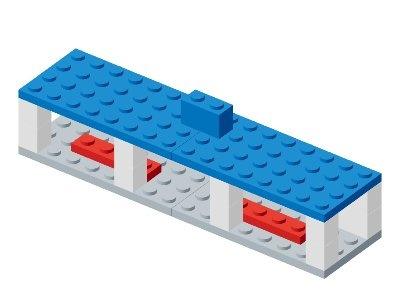
\includegraphics[width=.31\textwidth]{figures/review-cases/case-22-input.jpg} & 
\includegraphics[width=.31\textwidth]{figures/review-cases/case-22-good.jpg} & 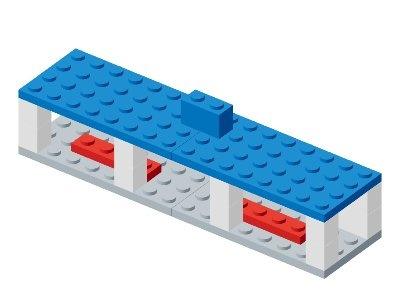
\includegraphics[width=.31\textwidth]{figures/review-cases/case-22-bad.jpg}\\
\end{tabular}\par
\noindent Strict success: positive $1$, negative $0$. Rejection: \texttt{target\_mismatch}.
Machine-readable inputs, both answers and all metrics are in \texttt{review-gallery/case-22.json}.
Field-answer cases use scene images for context only; a matching scene is not a correct field answer.
\clearpage
\subsection{Two-Tier Pagoda}
\noindent Source: \texttt{hard-two-tier-pagoda}.
Two cases share this source. Read numeric/graph answer fields alongside context-only images.
\paragraph{plan.} Case \texttt{de20e6915476e83efe0342d7}.\par
Given the full target, return all IDs in an executable vertical insertion order. The negative reverses the order.\par
\noindent\begin{tabular}{@{}ccc@{}}
Input / context & Positive reference & Constructed negative\\

\includegraphics[width=.31\textwidth]{figures/review-cases/case-23-input.jpg} & 
\includegraphics[width=.31\textwidth]{figures/review-cases/case-23-good.jpg} & 
\includegraphics[width=.31\textwidth]{figures/review-cases/case-23-bad.jpg}\\
\end{tabular}\par
\noindent Strict success: positive $1$, negative $0$. Rejection: \texttt{unsupported, incomplete}.
Machine-readable inputs, both answers and all metrics are in \texttt{review-gallery/case-23.json}.
Field-answer cases use scene images for context only; a matching scene is not a correct field answer.
\paragraph{repair.} Case \texttt{9e1b095a051a63df43d8d852}.\par
Given current and full symbolic reference, restore a wrong color and report its current ID. The negative copies current.\par
\noindent\begin{tabular}{@{}ccc@{}}
Input / context & Positive reference & Constructed negative\\

\includegraphics[width=.31\textwidth]{figures/review-cases/case-24-input.jpg} & 
\includegraphics[width=.31\textwidth]{figures/review-cases/case-24-good.jpg} & 
\includegraphics[width=.31\textwidth]{figures/review-cases/case-24-bad.jpg}\\
\end{tabular}\par
\noindent Strict success: positive $1$, negative $0$. Rejection: \texttt{target\_mismatch}.
Machine-readable inputs, both answers and all metrics are in \texttt{review-gallery/case-24.json}.
Field-answer cases use scene images for context only; a matching scene is not a correct field answer.
\clearpage
\subsection{Three-Span Truss Bridge}
\noindent Source: \texttt{expert-truss-bridge}.
Two cases share this source. Read numeric/graph answer fields alongside context-only images.
\paragraph{recovery-plan.} Case \texttt{4525bbe39009b121d8181a01}.\par
Recover from a legal but blocked deck-first state. Return remove/place actions that reach the complete target without reordering by the evaluator.\par
\noindent\begin{tabular}{@{}ccc@{}}
Input / context & Positive reference & Constructed negative\\
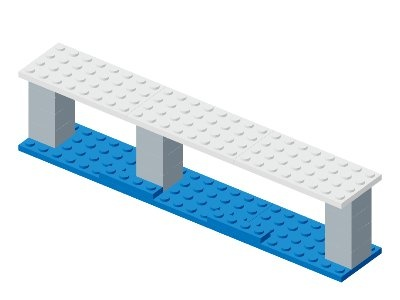
\includegraphics[width=.31\textwidth]{figures/review-cases/case-25-input.jpg} & 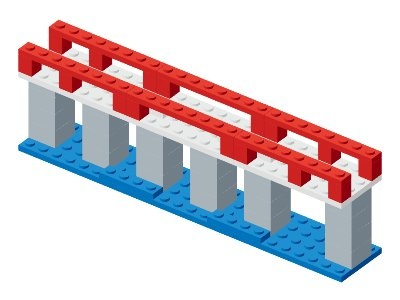
\includegraphics[width=.31\textwidth]{figures/review-cases/case-25-good.jpg} & 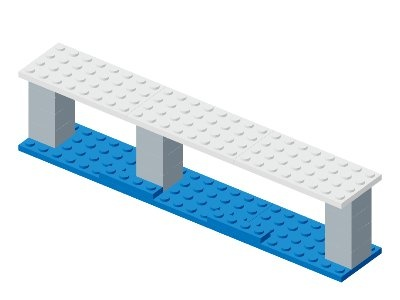
\includegraphics[width=.31\textwidth]{figures/review-cases/case-25-bad.jpg}\\
\end{tabular}\par
\noindent Strict success: positive $1$, negative $0$. Rejection: \texttt{illegal\_action}.
Machine-readable inputs, both answers and all metrics are in \texttt{review-gallery/case-25.json}.
Field-answer cases use scene images for context only; a matching scene is not a correct field answer.
\paragraph{support-counterfactual.} Case \texttt{03102cc267961f8f67a6c1fd}.\par
If the declared two support columns disappear simultaneously, report every additional piece removed by iterative loss of direct stud support.\par
\noindent\begin{tabular}{@{}ccc@{}}
Input / context & Positive reference & Constructed negative\\
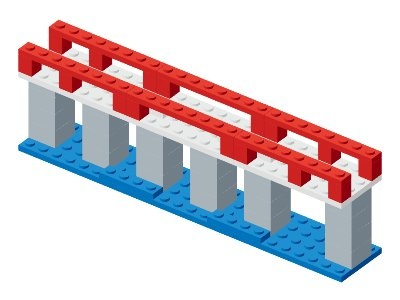
\includegraphics[width=.31\textwidth]{figures/review-cases/case-26-input.jpg} & 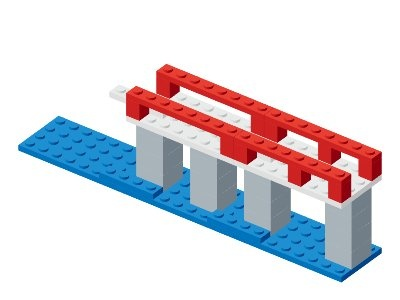
\includegraphics[width=.31\textwidth]{figures/review-cases/case-26-good.jpg} & 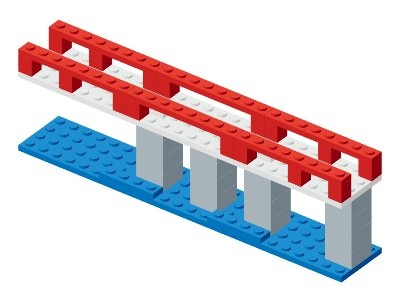
\includegraphics[width=.31\textwidth]{figures/review-cases/case-26-bad.jpg}\\
\end{tabular}\par
\noindent Strict success: positive $1$, negative $0$. Rejection: \texttt{set\_mismatch}.
Machine-readable inputs, both answers and all metrics are in \texttt{review-gallery/case-26.json}.
Field-answer cases use scene images for context only; a matching scene is not a correct field answer.
\begin{quote}\small
\begin{verbatim}
Positive: {"unsupportedIds": ["deck-1", "rail-1", "rail-4", "rail-post-1", "rail-post-10",
"rail-post-11", "rail-post-2", "rail-post-3", "rail-post-9"]}
Negative: {"unsupportedIds": []}
\end{verbatim}
\end{quote}
\clearpage
\subsection{Grand Railway Terminal}
\noindent Source: \texttt{expert-grand-terminal}.
Two cases share this source. Read numeric/graph answer fields alongside context-only images.
\paragraph{compound-edit.} Case \texttt{784592203ea29dc17078f9eb}.\par
Apply all clauses atomically: recolor the blue canopy red, remove bench-2 and bench-4, add the two specified yellow roof lights, and preserve every other part.\par
\noindent\begin{tabular}{@{}ccc@{}}
Input / context & Positive reference & Constructed negative\\
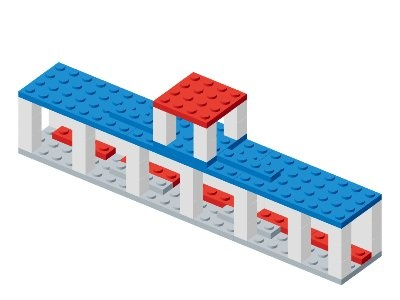
\includegraphics[width=.31\textwidth]{figures/review-cases/case-27-input.jpg} & 
\includegraphics[width=.31\textwidth]{figures/review-cases/case-27-good.jpg} & 
\includegraphics[width=.31\textwidth]{figures/review-cases/case-27-bad.jpg}\\
\end{tabular}\par
\noindent Strict success: positive $1$, negative $0$. Rejection: \texttt{target\_mismatch}.
Machine-readable inputs, both answers and all metrics are in \texttt{review-gallery/case-27.json}.
Field-answer cases use scene images for context only; a matching scene is not a correct field answer.
\paragraph{multi-fault-repair.} Case \texttt{e8c2121ecc177d0237e011dd}.\par
Repair three simultaneous faults: one recolor, one shifted part, and one extra part. Return the corrected structure and all wrong CURRENT IDs. Layer disclosure is supplied: recover complete geometry up to piece yaw symmetry, not exterior RGB alone.\par
\noindent\begin{tabular}{@{}ccc@{}}
Input / context & Positive reference & Constructed negative\\
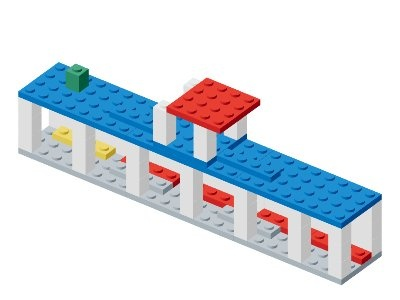
\includegraphics[width=.31\textwidth]{figures/review-cases/case-28-input.jpg} & 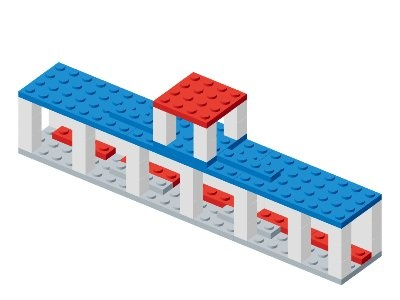
\includegraphics[width=.31\textwidth]{figures/review-cases/case-28-good.jpg} & 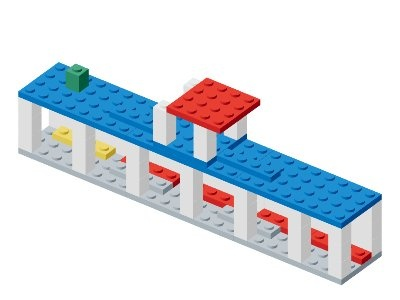
\includegraphics[width=.31\textwidth]{figures/review-cases/case-28-bad.jpg}\\
\end{tabular}\par
\noindent Strict success: positive $1$, negative $0$. Rejection: \texttt{target\_mismatch, fault\_mismatch}.
Machine-readable inputs, both answers and all metrics are in \texttt{review-gallery/case-28.json}.
Field-answer cases use scene images for context only; a matching scene is not a correct field answer.
\clearpage
\subsection{Fortress Gatehouse}
\noindent Source: \texttt{expert-fortress-gatehouse}.
Two cases share this source. Read numeric/graph answer fields alongside context-only images.
\paragraph{active-inspection.} Case \texttt{6f5b964a86860cd2e99722de}.\par
Select a query, read its returned observation, then report how many parallel rows the white gate beams occupy. Each row can contain multiple beam parts. Success requires a layer-disclosing query; cost is scored separately, not an optimality proof.\par
\noindent\begin{tabular}{@{}ccc@{}}
Input / context & Positive reference & Constructed negative\\
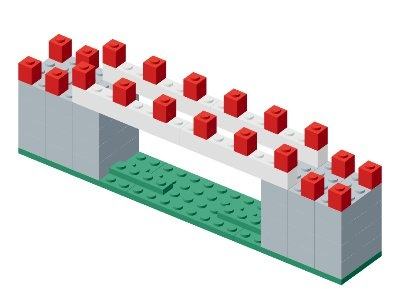
\includegraphics[width=.31\textwidth]{figures/review-cases/case-29-input.jpg} & 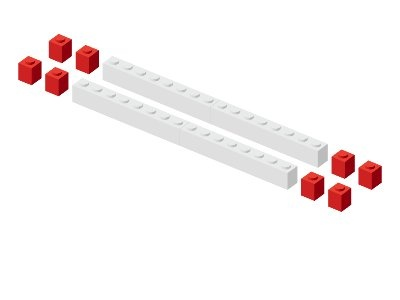
\includegraphics[width=.31\textwidth]{figures/review-cases/case-29-good.jpg} & 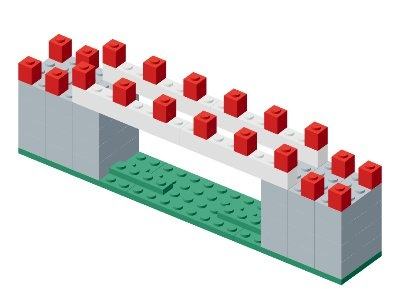
\includegraphics[width=.31\textwidth]{figures/review-cases/case-29-bad.jpg}\\
\end{tabular}\par
\noindent Strict success: positive $1$, negative $0$. Rejection: \texttt{answer\_mismatch}.
Machine-readable inputs, both answers and all metrics are in \texttt{review-gallery/case-29.json}.
Field-answer cases use scene images for context only; a matching scene is not a correct field answer.
\begin{quote}\small
\begin{verbatim}
Positive: {"queryId": "layer-y-13", "answer": "two-parallel-beams"}
Negative: {"queryId": "unknown", "answer": "two-parallel-beams"}
\end{verbatim}
\end{quote}
\paragraph{graph-reasoning.} Case \texttt{2057760ea52daf7c9b82ccb3}.\par
Return the shortest stud-contact path length between the queried merlons and every articulation piece in the full contact graph.\par
\noindent\begin{tabular}{@{}ccc@{}}
Input / context & Positive reference & Constructed negative\\
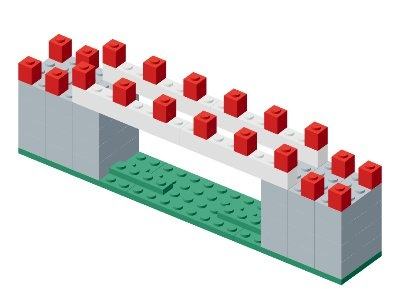
\includegraphics[width=.31\textwidth]{figures/review-cases/case-30-input.jpg} & 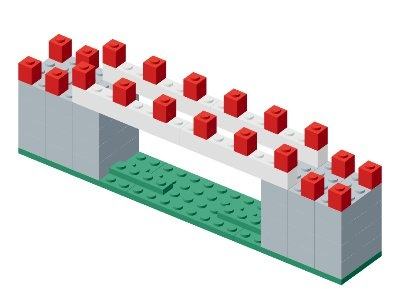
\includegraphics[width=.31\textwidth]{figures/review-cases/case-30-good.jpg} & 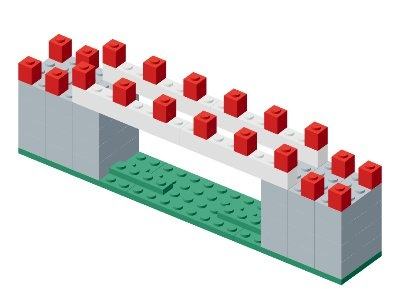
\includegraphics[width=.31\textwidth]{figures/review-cases/case-30-bad.jpg}\\
\end{tabular}\par
\noindent Strict success: positive $1$, negative $0$. Rejection: \texttt{answer\_mismatch}.
Machine-readable inputs, both answers and all metrics are in \texttt{review-gallery/case-30.json}.
Field-answer cases use scene images for context only; a matching scene is not a correct field answer.
\begin{quote}\small
\begin{verbatim}
Positive: {"shortestPath": 14, "articulationIds": ["base-1", "base-2", "base-3", "base-
seam-1", "base-seam-2", "gate-beam-1", "gate-beam-2", "gate-beam-3", "gate-beam-4",
"tower-1", "tower-10", "tower-11", "tower-12", "tower-13", "tower-14", "tower-15",
"tower-16", "tower-17", "tower-18", "tower-19", "tower-2", "tower-20", "tower-21",
"tower-22", "tower-23", "tower-24", "tower-3", "tower-4", "tower-5", "tower-6", "tower-7",
"tower-8", "tower-9"]}
Negative: {"shortestPath": 15, "articulationIds": ["base-1", "base-2", "base-3", "base-
seam-1", "base-seam-2", "gate-beam-1", "gate-beam-2", "gate-beam-3", "gate-beam-4",
"tower-1", "tower-10", "tower-11", "tower-12", "tower-13", "tower-14", "tower-15",
"tower-16", "tower-17", "tower-18", "tower-19", "tower-2", "tower-20", "tower-21",
"tower-22", "tower-23", "tower-24", "tower-3", "tower-4", "tower-5", "tower-6", "tower-7",
"tower-8", "tower-9"]}
\end{verbatim}
\end{quote}
\clearpage
\subsection{Stepped Temple Complex}
\noindent Source: \texttt{advanced-stepped-temple}.
Two cases share this source. Read numeric/graph answer fields alongside context-only images.
\paragraph{distributed-completion.} Case \texttt{0482601199de9b79b7208a9d}.\par
Restore eight missing columns distributed across both tiers. Preserve every supplied part exactly; the missing region is not a suffix. Layer disclosure is supplied: recover complete geometry up to piece yaw symmetry, not exterior RGB alone.\par
\noindent\begin{tabular}{@{}ccc@{}}
Input / context & Positive reference & Constructed negative\\

\includegraphics[width=.31\textwidth]{figures/review-cases/case-31-input.jpg} & 
\includegraphics[width=.31\textwidth]{figures/review-cases/case-31-good.jpg} & 
\includegraphics[width=.31\textwidth]{figures/review-cases/case-31-bad.jpg}\\
\end{tabular}\par
\noindent Strict success: positive $1$, negative $0$. Rejection: \texttt{target\_mismatch}.
Machine-readable inputs, both answers and all metrics are in \texttt{review-gallery/case-31.json}.
Field-answer cases use scene images for context only; a matching scene is not a correct field answer.
\paragraph{module-transplant.} Case \texttt{1ed677903af5f888740674f9}.\par
Move the complete upper pavilion four studs toward +X as a rigid module. Preserve its internal layout and every lower-tier part.\par
\noindent\begin{tabular}{@{}ccc@{}}
Input / context & Positive reference & Constructed negative\\

\includegraphics[width=.31\textwidth]{figures/review-cases/case-32-input.jpg} & 
\includegraphics[width=.31\textwidth]{figures/review-cases/case-32-good.jpg} & 
\includegraphics[width=.31\textwidth]{figures/review-cases/case-32-bad.jpg}\\
\end{tabular}\par
\noindent Strict success: positive $1$, negative $0$. Rejection: \texttt{target\_mismatch}.
Machine-readable inputs, both answers and all metrics are in \texttt{review-gallery/case-32.json}.
Field-answer cases use scene images for context only; a matching scene is not a correct field answer.
\clearpage
\subsection{Double-Deck Aqueduct}
\noindent Source: \texttt{expert-double-deck-aqueduct}.
Two cases share this source. Read numeric/graph answer fields alongside context-only images.
\paragraph{step-selection.} Case \texttt{c5ba6f85a9a06e3162407ac6}.\par
Select every candidate that can legally be inserted next into the current partial aqueduct. Do not use the target order as an answer.\par
\noindent\begin{tabular}{@{}ccc@{}}
Input / context & Positive reference & Constructed negative\\
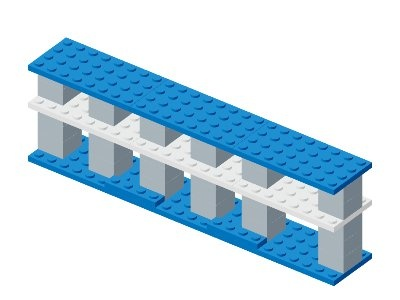
\includegraphics[width=.31\textwidth]{figures/review-cases/case-33-input.jpg} & 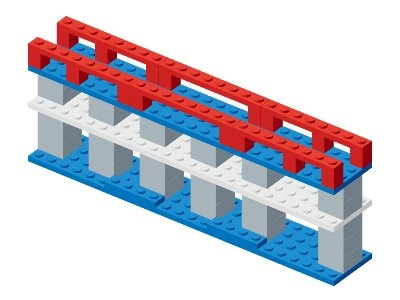
\includegraphics[width=.31\textwidth]{figures/review-cases/case-33-good.jpg} & 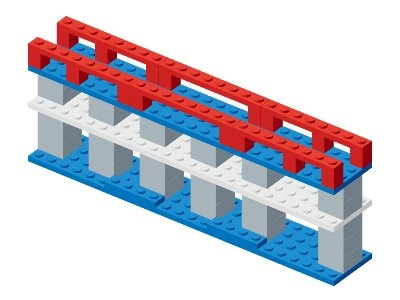
\includegraphics[width=.31\textwidth]{figures/review-cases/case-33-bad.jpg}\\
\end{tabular}\par
\noindent Strict success: positive $1$, negative $0$. Rejection: \texttt{selection\_mismatch}.
Machine-readable inputs, both answers and all metrics are in \texttt{review-gallery/case-33.json}.
Field-answer cases use scene images for context only; a matching scene is not a correct field answer.
\begin{quote}\small
\begin{verbatim}
Positive: {"legalIds": ["parapet-post-1", "parapet-post-2", "parapet-post-3", "parapet-
post-4", "parapet-post-5", "parapet-post-6"]}
Negative: {"legalIds": []}
\end{verbatim}
\end{quote}
\paragraph{pose-estimation.} Case \texttt{e4d1526119eb949e17077c01}.\par
Place the selected parapet post into its target pose from the current state and reference views; accept equivalent yaw for its footprint.\par
\noindent\begin{tabular}{@{}ccc@{}}
Input / context & Positive reference & Constructed negative\\
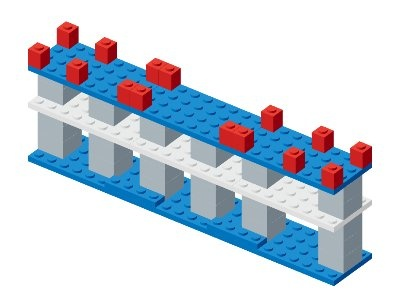
\includegraphics[width=.31\textwidth]{figures/review-cases/case-34-input.jpg} & 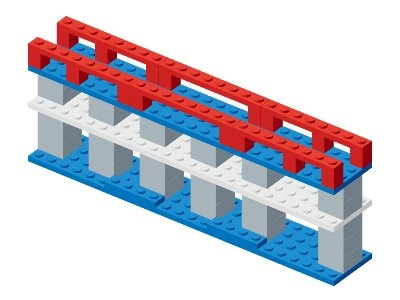
\includegraphics[width=.31\textwidth]{figures/review-cases/case-34-good.jpg} & 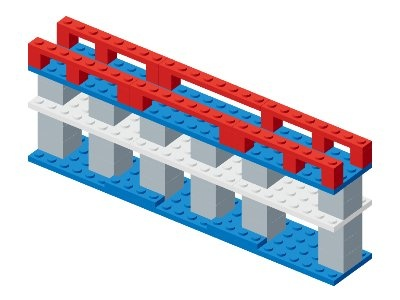
\includegraphics[width=.31\textwidth]{figures/review-cases/case-34-bad.jpg}\\
\end{tabular}\par
\noindent Strict success: positive $1$, negative $0$. Rejection: \texttt{answer\_mismatch}.
Machine-readable inputs, both answers and all metrics are in \texttt{review-gallery/case-34.json}.
Field-answer cases use scene images for context only; a matching scene is not a correct field answer.
\begin{quote}\small
\begin{verbatim}
Positive: {"x": 15, "y": 18, "z": 0, "turn": 0}
Negative: {"x": 16, "y": 18, "z": 0, "turn": 0}
\end{verbatim}
\end{quote}
\clearpage
\subsection{Covered Market Hall}
\noindent Source: \texttt{advanced-covered-market}.
Two cases share this source. Read numeric/graph answer fields alongside context-only images.
\paragraph{scene-reconstruction.} Case \texttt{770a5b457843640c815ff8ef}.\par
Reconstruct the complete 53-part market from four views and its bill of materials. Repeated columns and signs remain distinct instances. Layer disclosure is supplied: recover complete geometry up to piece yaw symmetry, not exterior RGB alone.\par
\noindent\begin{tabular}{@{}ccc@{}}
Input / context & Positive reference & Constructed negative\\
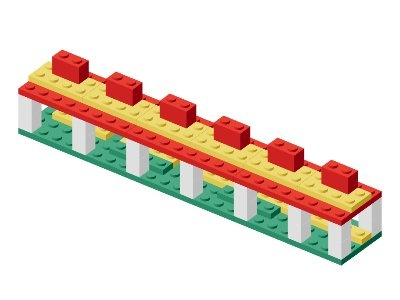
\includegraphics[width=.31\textwidth]{figures/review-cases/case-35-input.jpg} & 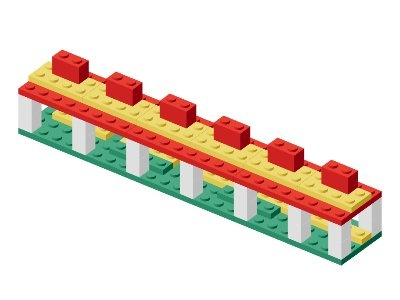
\includegraphics[width=.31\textwidth]{figures/review-cases/case-35-good.jpg} & 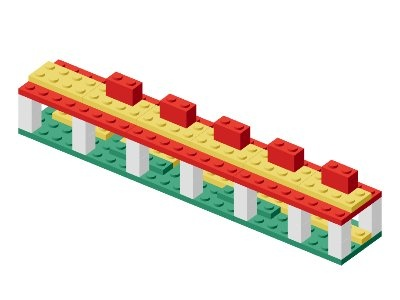
\includegraphics[width=.31\textwidth]{figures/review-cases/case-35-bad.jpg}\\
\end{tabular}\par
\noindent Strict success: positive $1$, negative $0$. Rejection: \texttt{target\_mismatch}.
Machine-readable inputs, both answers and all metrics are in \texttt{review-gallery/case-35.json}.
Field-answer cases use scene images for context only; a matching scene is not a correct field answer.
\paragraph{constrained-redesign.} Case \texttt{320d35b94f077a31b364afa0}.\par
Design any connected grid structure preserving the foundation, within inventory and exact extent, with at least four colors and minRoofCells occupied 3D cells among parts whose bottom Y>=7. This measures a volume proxy, not semantic roof coverage.\par
\noindent\begin{tabular}{@{}ccc@{}}
Input / context & Positive reference & Constructed negative\\

\includegraphics[width=.31\textwidth]{figures/review-cases/case-36-input.jpg} & 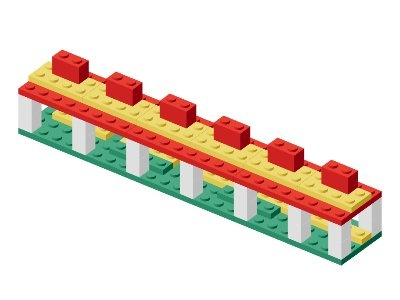
\includegraphics[width=.31\textwidth]{figures/review-cases/case-36-good.jpg} & 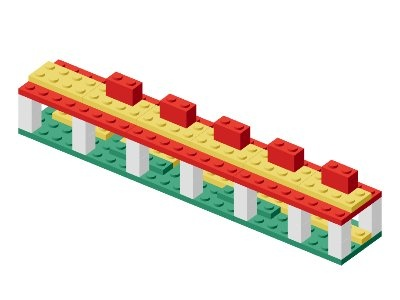
\includegraphics[width=.31\textwidth]{figures/review-cases/case-36-bad.jpg}\\
\end{tabular}\par
\noindent Strict success: positive $1$, negative $0$. Rejection: \texttt{roofCoverage}.
Machine-readable inputs, both answers and all metrics are in \texttt{review-gallery/case-36.json}.
Field-answer cases use scene images for context only; a matching scene is not a correct field answer.
